\section{Our Approach}
\label{sec:approach}

We first present an overview of our approach. Then, we propose the underlying data model. The data model introduces the requirement \hlc{of the} techniques to represent the POIs and the POSes. We illustrate how our approach address this problem at last.

\subsection{Overview}
\todo{this section need rewriting. focus on data.}
\begin{figure}
\begin{center}
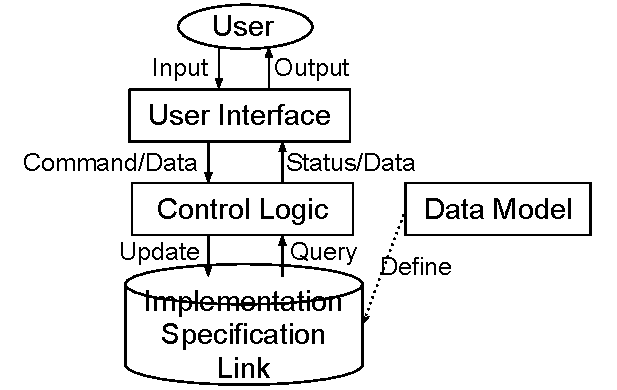
\includegraphics[width=0.55\textwidth]{framework}
\caption{Framework of Our Approach.}
\label{fig:framework}
\end{center}
\end{figure}

As shown in Fig.~\ref{fig:framework}, the framework of our approach consists three components: database, control logic, and user interface. The structure of the traceability link data in the database is defined by the data model. Control logic lays in the middle of user interface and datamodel. It receives and processes command from the user interface. Depending on the command, it either updates the database, or queries the data in the database and report the result to the user interface. User interface is responsible of communicating with the end user, processs and passes the input from user to the control logic, get the result from the control logic and present the result to the user.



\begin{figure}
\begin{center}
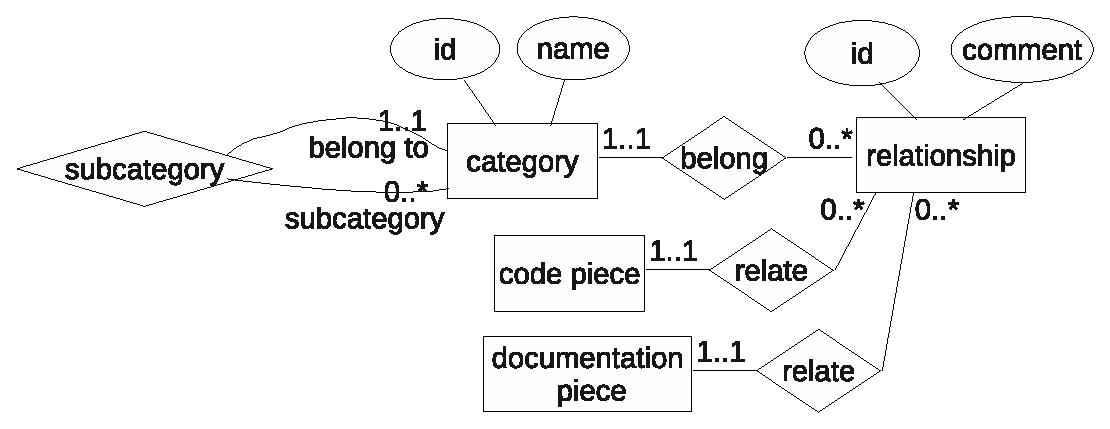
\includegraphics[width=0.85\textwidth]{datamodel}
\caption{Data Model. Entity-Relation Model is used. Rectangles represent entity sets. Ovals represent attributes. Diamonds represent relationships.}
\label{fig:datamodel}
\end{center}
\end{figure}

\subsection{Data Model}
The data model is the key to support fine-grained links between basic elements of specifications and semantic constructs of implementation languages and automatic migration of links as implementations evolve. We introduce the data model of our approach in this section.

The data model describes the data objects being handled in the framework, their attributes, and the relationships between these data objects.
Fig.~\ref{fig:datamodel} presents the data model of our design.
Entiry-relationship model is used.
Rectangles represent entiry sets.
Ovals represent attributes.
Diamonds represent relationships.
We have four entity sets in our design: code file mark, spec file mark, code piece anchor and specification piece anchor.
Code piece anchor and specification piece anchor represent the selected code and specification piece respectively.
Both code file mark and spec file mark entities have attributes id and path:
id is a 128-bit number, and serves as the key of the entity;
path is the file path pointing to a file in the local machine. % not a key, it may change
Code piece anchor and spec piece anchor have id and path as attributes:
id is a 128-bit number, and serves as the key;
path points to the code or spec piece.
Traceability links are represented by the relationships between code piece anchor and spec piece anchor.

Special attention should be paid to four attributes: path for code file, path for spec file, path for code piece anchor and path for spec piece anchor.
\todo{explain}\hlc{These four attributes are foreign keys used to refer to data that do not exist in database.}
As foreign keys, these attributes should be able to uniquely identify the entities they refer to.
The path provided by the file system is a solution to the path for code files and spec files, as we can easily identify both code files and spec files by these pathes.
The pathes for anchors are challenging, little work has been done to address this problem.

%Based on the model above, we can conclude the schema as following.
%Examples?

\subsection{Anchor Design}

Anchors includes specification anchor and implementation anchor. The three basic requirements for traceability links are the constraints for the design. We present how our approach make these requirements fulfilled. Specification anchor design is addressed first, then we present the implementation anchor design.

\subsubsection{Spec Anchor}

Specifications are relatively stable, which make the specification anchor design easier than implementation anchor. Using the absolute coordinate is enough to meet the requirements. Most of the HW/SW interface specification are in PDF format. We use this format to present our approach. Basically, the coordinate for specification piece is denoted by two points -- the point representing the beginnings of the selection and the point representing the end of the selection. Each point is denoted by a vector $<$page, x-coord, y-coord$>$, where page is the page number the point located, x-coord and y-coord are the horizontal and vertical coordinate respectively.

The method is accurate as each point is uniquely represented by the coordinate. This method is also fine-grained, because this method could represent each word, sentence or evan arbitrary size of POS. The method is not robust as it uses the absolute coordinate as the basic element of the anchor. However, specifications are relatively stable, which makes this approach work most of the time.


\subsubsection{Offset-Based Anchor}

Similar to specification anchor,
absolute coordinates also fit the situation of implementation anchor.
Basically, implementation code is just a string of ASCII charactors. 
Each piece of code is a substring of this string.
We can use the offset of the substring in the string and the length of the piece of code to represent this piece of code.
The pair (offset, length) is called Offset-Based Anchor.
Fig.~\ref{fig:code}(a) illustrate this technique.
The parenthesized number in front of each line represent the offset of the first charactor of that line.
Using this approach, we can get the Offset-Based Anchors for the three code pieces labeled 1, 2 and 3 as (590, 4), (614, 4) and (635, 4) respectively.

The advantage of this technique is obvious, it is simple and provides fine-grained traceability. The disadvantage of this technique is that these anchors fail after the code evolves. Fig.~\ref{fig:code}(b) is the code after the code in Fig.~\ref{fig:code}(a) evolves. We can see the anchors we get above do not point to the previous pieces of code anymore. The reason is that this approach is context sensitive. By saying context sensitive, we mean it depends on its context. In this approach, the anchor depends on the number of charactors preceeding the piece of code.

One way to overcome this disadvantage is to get the knowledge of change to keep the links valid. However, this information is not always available. Most of the time, code is changed by other people. We can only get the changed result without how the change is made.

% a figure example
\begin{figure}[h!]
  \begin{center}
    \begin{tabular}{c}
\begin{minipage}[b]{\linewidth}
  \centering
  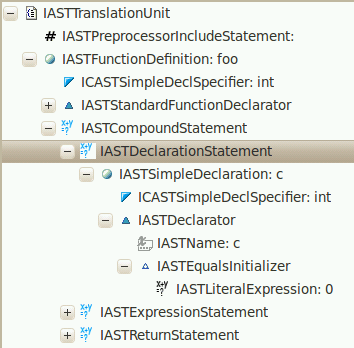
\includegraphics[width=0.8\linewidth]{ast1}
\end{minipage}\\
(a) AST for the Code in Fig.~\ref{fig:code}(a)\\
\\
\begin{minipage}[b]{\linewidth}
  \centering
  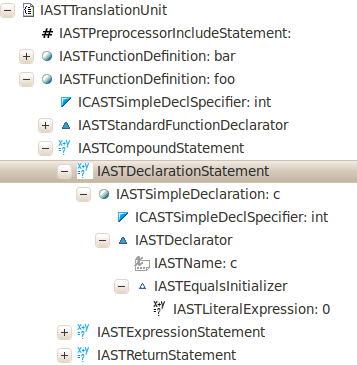
\includegraphics[width=0.8\linewidth]{ast2}
\end{minipage}\\
(b) AST for the Code in Fig.~\ref{fig:code}(b)\\
\\
\begin{minipage}[b]{\linewidth}
  \centering
  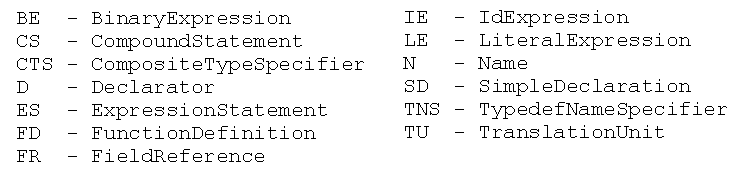
\includegraphics[width=0.95\linewidth]{ast_legend}
\end{minipage}
\end{tabular}
\caption{The AST for the implementation code in Fig.~\ref{fig:code}.}
\label{fig:ast}
\end{center}
\end{figure}

% syntax tree, a string of syntax tree leaf nodes.
% content-free (make immune from change of the content) vs content-sensitive (make unique)
% evaluate on unique
\subsubsection{Syntax Tree Based Anchor}
To make the traceability links created for one version of code work for other versions,
we need a robust strategy to represent the code pieces.
More specifically, we need to find some properties of the code that are relatively stable when code evolves.
These properties can serve as keys to identify the code piece.
We use syntax information to form the main element of our code piece identifier.
The code can be parsed and represented by a parse tree or an abstract syntax tree (AST).
We use AST in our approach, as it faithfully retains the structure of the original source code, and is concise and efficient to compute compared to parse tree.
AST usually has fewer nodes than parse tree, and takes less time to traverse.
Each node in AST tree represents a syntax unit of the grammer,
a parent of a node represent a bigger grammer unit that includes the grammer unit represented by the child node.
The nodes are labeled by the type of the grammer unit.
For each leaf node, we also include the value, which is the code this node represents, in the label.
For some of the inner nodes that have a name, we also include the name in their labels. For example, a inner node that represents a function will be labeled with the grammer unit type and the name of the function.
A change of the code in one branch of AST usually does not affect the structure in other branches.
Representing code pieces based on the structure in the syntax tree is robust.
Fig.~\ref{fig:ast}(a) and Fig.~\ref{fig:ast}(b) are the Abstract Syntax Trees (AST) for the code in Fig.~\ref{fig:code}(a) and Fig.~\ref{fig:code}(b).
Dot lines represent branches not shown.
Fig.~\ref{fig:ast}(a) shows two subtrees of the root.
The left subtree represents line 13 - line 25 of Fig.~\ref{fig:code}(a), which defines the structure max7310\_s.
The right subtree represent line 27 - line 35 of Fig.~\ref{fig:code}(a), which defines the function max7310\_reset.
Similarly, the left subtree of the AST in Fig.~\ref{fig:ast}(b) represent line 12 - line 24 in Fig.~\ref{fig:code}(b), and the right subtree represents line 26 - line 34.
From the AST shown in Fig.~\ref{fig:ast}(a) and fig.~\ref{fig:ast}(b), we can see that the left tree has changed as the code for structure definition changed.
However, the structure of the right subtree remain the same, unaffected by the change of the left subtree.

Based on the AST of the code, we define our identifier to a piece of code as a sequence of leaf nodes in the AST. Each leaf node is represented by the path from the leaf node to the root of the AST. For example, line 31 in Fig.~\ref{fig:code}(a) is represented by the highlighted three leaf nodes in Fig.~\ref{fig:ast}(a). The leaf nodes are in the same order as they are visited by depth-first search of the AST. For this example, the closest common parent node for these three leaf nodes also represents the same piece of code, and thes representation is even simpler. We avoid using this representation for two reasons: First, this representation contains less information; Second, this representation is sensitive to formatting and style convention. For example, some programmer may prefer no spaces adjacent to the equal sign, or they may insert some spaces besides the equal sign to make it aligned with other lines of assignment statements. Either case will change the string represented by this common parent, and make the traceability link invalid. We will address how we determine if a traceability link is valid or not in the next section.

Using this approach, let's consider the pieces of code label by 1, 2 and 3 in fig.~\ref{fig:code} again. The identifier for these code pieces in AST are shown in fig.~\ref{fig:ast} labeled with the same number.
Through the two ASTs are different, 
the highlighted nodes can be represented by the same path from the roots of these two ASTs.
As a result, we can use this method to identify the piece of code, and the change of the unrelated code does not invalidate the identifier.

This method is relatively stable.
However, it may not uniquely identify a piece of code,
which means one identifier may refer to two or more pieces of code.
The pieces of code label by 1 and 3 in fig.~\ref{fig:ast}(a) showes two pathes that are encoded as the same identifier -- $<$\texttt{LE:0xff/BE/ES/CS/FD:max7310\_reset/TU}$>$.
As a result, this identifier can not distinguish these two pieces of code, 
and can not serve as a key to these pieces of code.

\subsubsection{Hybrid Anchor}

Offset-based anchor can uniquely identify a piece of code, but it is not immune to code evolusion.
Syntax tree based anchor is immune to code evolusion, but it can not uniquely identify some pieces of code.
We combine these two methods and form hybrid anchor.
For each leaf node that has an ambiguous path representation,
we can always find at least one of its ancesters that has an unique path.
In the worst case, we will get to the root node.
Our approach is composed of two steps.
First, we compute the syntax tree based anchor,
then, we go over the path from leaf to root, find the first node that is a unique identifier.
Second, we compute offset based anchor based on this unique identifier instead of the begining of the whole implementation code.
Consider the AST in fig.~\ref{fig:ast}(a), to identify the piece of code labeled by 1,
we go through the path towards the root,
and get to the first unique identifier at the inner node CS.
The node CS represent line 28 - line 35 of the code in fig.~\ref{fig:code}(a).
It is the body of the function \texttt{max7310\_reset}, and there is only one body for this function by the C language grammer.
The offset based identifier based on this node is (103,4), as the first charactor of the node CS is located at offset 487 and the offset based anchor is (590,4).
We combine the information of the inner node CS and the calculated coordinate to represent the piece of code with no ambiguity.
Same as offset based anchor, if the code does not change, it can uniquely identify the piece of code.
If the code changes, this method still works if the code for the unique identifier remain the same.
Actually, this is a general approach for the previous two.
If we get to the root node while finding the first unique ancestor, then this approach will become the same as offset based anchor.
However, if the lead node itself is the firtst node with unique identifier, then this approach is the same as syntax based anchor.
The lower the node with the unique identifier in AST, the better our approach works.
%However, this method provide redundent information, which can be used to check the validity.

% example?
